\documentclass[12pt]{article}

\usepackage{amssymb, amsmath, amsfonts}
\usepackage{amsthm}
\usepackage{moreverb}
\usepackage{graphicx}
\usepackage{enumerate}
\usepackage{graphics}
\usepackage{color}
\usepackage{array}
\usepackage{float}
\usepackage{hyperref}
\usepackage{textcomp}
\usepackage{alltt}
\usepackage{mathtools}
\usepackage[T1]{fontenc}
\usepackage{fullpage}
\usepackage{tikz}
\usepackage[utf8]{inputenc}
\newcommand{\suchthat}{\, \mid \,}
\usepackage{fancyvrb}
\newenvironment{qv}
{\quote\Verbatim}
{\endVerbatim\endquote}
%\allowdisplaybreaks
\def\arraystretch{1.7}%  1 is the default, change whatever you need

\begin{document}

{\bf MATH 481A \hfill Numerical Analysis \ \ \ \ \ \hfill Spring 2015}

\title{\bf Lab \# 1 Solutions}
\author{\bf Sam Fleischer}
\date{\bf Thurs. Feb. 5, 2015}

{\let\newpage\relax\maketitle}
\maketitle
\tableofcontents
\pagebreak

\section*{Problem 1}
\addcontentsline{toc}{section}{Problem 1}

The following Python function was used to find the value of {\it machine epsilon}, the largest floating point number, $\epsilon$, such that $1 \oplus \epsilon = 1$.
\begin{qv}
def machineEpsilon(func = float):
    machine_epsilon = func(1)
    while func(1) + func(machine_epsilon) != func(1):
        machine_epsilon_last = machine_epsilon
        machine_epsilon = func(machine_epsilon) / func(2)
    return machine_epsilon_last
\end{qv}
The Python command line environment in Canopy produced the following:
\begin{qv}
In : machineEpsilon()
Out: 2.220446049250313e-16
\end{qv}
Thus $\boxed{\epsilon = 2.220446049250313 \times 10^{-16}}$

\section*{Problem 2}
\addcontentsline{toc}{section}{Problem 2}

According to online sources, the smallest (by absolute value) floating point number for a double precision system using the IEEE 754 standard is $1 \times 10^{-101}$.  The largest (by abosolute value) floating point number for a double precision system using the same standards is $9.999999 \times 10^{96}$.  Thus the full range for this system is $[-9.999999 \times 10^{96}, 9.999999 \times 10^{96}]$.

\section*{Problem 3}
\addcontentsline{toc}{section}{Problem 3}

The formula
\begin{align*}
f'(x) \approx \frac{f(x + h) - f(x - h)}{2h}
\end{align*}
is used to approximate the derivate of a function $f(x)$.  The following Python function was used to approximate the derivative of $f(x) = \ln x$ at $ x = 10$ for various values of $h$.
\begin{qv}
def deriv_approx(f, x, h):
    numer = f(x + h) - f(x - h)
    denom = 2*h
    return numer/denom
\end{qv}
The Python command line environment in Canopy produced the following:
\begin{qv}
In : hs = [0.5, 0.1, 10**-3, 10**-5, 10**-7, 10**-9, 10**-11]

In : for h in hs:
...:    d = double_der(math.log, 10, h)
...:    print("h=%.11f gives f'(x) is approx. %.15f" % (h, d))
...:    
h=0.50000000000 gives f'(x) is approx. 0.100083458556982
h=0.10000000000 gives f'(x) is approx. 0.100003333533347
h=0.00100000000 gives f'(x) is approx. 0.100000000333278
h=0.00001000000 gives f'(x) is approx. 0.099999999991773
h=0.00000010000 gives f'(x) is approx. 0.099999999392253
h=0.00000000100 gives f'(x) is approx. 0.100000008274037
h=0.00000000001 gives f'(x) is approx. 0.099986685597742
\end{qv}
The following table is a summary of the above information.  Note $f(x) = \ln x \\ \implies f'(x) = \dfrac{1}{x} \implies f'(10) = 0.1$.
\begin{table}[H]
    \centering
    \begin{tabular}{|l|l|l|l|}
    & \multicolumn{1}{c|}{\bf Approximation} & \multicolumn{1}{c|}{\bf Absolute Error} & \multicolumn{1}{c|}{\bf Relative Error} \\
    \multicolumn{1}{|c|}{$h$} & \multicolumn{1}{c|}{$\overline{N}$} & \multicolumn{1}{c|}{$|E| = |0.1 - \overline{N}|$} & \multicolumn{1}{c|}{$|R| = \left|\dfrac{E}{0.1}\right|$}\\ [.2cm] \hline
    $0.5$ & $0.100083458556982$ & $8.34585569823\times 10^{-5}$ & $8.34585569823\times10^{-4}$ \\ \hline
    $0.1$ & $0.100003333533347$ & $3.33353334722\times 10^{-6}$ & $3.33353334722\times 10^{-5}$ \\ \hline
    $10^{-3}$ & $0.100000000333278$ & $3.33277933029\times 10^{-10}$ & $3.33277933029\times 10^{-9}$ \\ \hline
    $10^{-5}$ & $0.099999999991773$ & $8.22668322353\times 10^{-12}$ & $8.22668322353\times 10^{-11}$ \\ \hline
    $10^{-7}$ & $0.099999999392253$ & $6.07747102643\times 10^{-10}$ & $6.07747102643\times 10^{-9}$ \\ \hline
    $10^{-9}$ & $0.100000008274037$ & $8.27403709436\times 10^{-9}$ & $8.27403709436\times 10^{-8}$ \\ \hline
    $10^{-11}$ & $0.099986685597742$ & $1.33144022584\times 10^{-5}$ & $1.33144022584\times 10^{-4}$ \\ \hline
    \end{tabular}
\end{table}

\begin{enumerate}[\ \ (a)\ \ ]
\addcontentsline{toc}{subsection}{(a)}
\item The $h \rightarrow 0$, the approximation get more accurate initially, but then diverges.  This is shown in the {\bf Absolute Error} and {\bf Relative Error} columns above.
\addcontentsline{toc}{subsection}{(b)}
\item The value of $h$ by which we get the smallest relative error is $10^{-5}$, and the value of $h$ by which we get the largest relative error is $0.5$.
\addcontentsline{toc}{subsection}{(c)}
\item In mathematical theory, the approximation of $f'(x)$ becomes more accurate as $h \rightarrow 0$.  Computers, however, cannot accurately store irrational numbers, or even certain rational numbers if their decimal value is repeated or too long.  This may be the reason for the increase in error as $h \rightarrow 0$.
\end{enumerate}

\section*{Problem 4}
\addcontentsline{toc}{section}{Problem 4}

The following Python functions were used to find the values of the roots of a polynomial.
\begin{qv}
import math
from mpmath import mp

def quadratic(a,b,c):
    if (b**2 - 4*a*c) < 0:
        return "Negative Discriminant: no real roots"
    else:
        x1 = (-b - math.sqrt(b**2 - 4*a*c))/(2.0*a)
        x2 = (-b + math.sqrt(b**2 - 4*a*c))/(2.0*a)
        return x1, x2

def quadratic_mp(a,b,c,n):
    mp.dps = n
    a = mp.mpf(a)
    b = mp.mpf(b)
    c = mp.mpf(c)
    b2 = mp.mpf(b*b)
    ac4 = mp.mpf(4*a*c)
    d = mp.mpf(b2-ac4)
    d = mp.sqrt(d)
    num1 = mp.mpf(-b-d)
    num2 = mp.mpf(-b+d)
    denom = mp.mpf(2.0*a)

    x1 = mp.mpf(num1/denom)
    x2 = mp.mpf(num2/denom)
    return x1, x2
\end{qv}

\begin{enumerate}[\ (a)\ ]
\item \addcontentsline{toc}{subsection}{(a)}
The Python command line environment was used to calculate the roots, without specification of the number of significant figures, of $ax^2 + bx + c = 0$ where $a = 1$, $b = 200$, and $c = -0.000015$.
\begin{qv}
In : a = 1; b = 200; c = -0.000015

In : quadratic(a, b, c)
Out: (-200.000000075, 7.500000265281415e-08)
\end{qv}
Thus the zeros of $ax^2 + bx + c = 0$ where $a = 1$, $b = 200$, and $c = -0.000015$, and without specification of the number of significant figures, are $\boxed{-200.000000075}$, and $\boxed{7.500000265281415\times 10^{-08}}$.

\item \addcontentsline{toc}{subsection}{(b)}
The Python command line environment was used to calculate the roots, using $10$ significant figures, of $ax^2 + bx + c = 0$ where $a = 1$, $b = 200$, and $c = -0.000015$.
\begin{qv}
In : a = 1; b = 200; c = -0.000015; n = 10

In : quadratic_mp(a, b, c, n)
Out: (mpf('-200.0000000745'), mpf('7.543712854385e-8'))
\end{qv}
Thus the zeros of $ax^2 + bx + c = 0$ where $a = 1$, $b = 200$, and $c = -0.000015$, and calculated using $10$ significant figures, are $\boxed{-200.0000000745}$, and $\boxed{7.543712854385\times 10^{-08}}$.

\item \addcontentsline{toc}{subsection}{(c)}
Let $a = 1$, $b = -1.786737601482363$, and $c = 2.054360090947453\times 10^{-8}$.
\begin{enumerate}[\ (i) \ ]
\item The Python command line environment was used to calculate the roots of $ax^2 + bx + c = 0$ without specification of the number of significant figures.
\begin{qv}
In : a = 1

In : b = -1.786737601482363

In : c = 2.054360090947453*(10**(-8))

In : quadratic(a, b, c)
Out: (1.1497827689943563e-08, 1.7867375899845355)
\end{qv}
Thus the zeros of $ax^2 + bx + c = 0$ where $a = 1$, $b = -1.786737601482363$, and $c = 2.054360090947453\times 10^{-8}$, and without the specification of the number of significant figures, are $\boxed{1.1497827689943563\times 10^{-8}}$, and $\boxed{1.7867375899845355}$.

\item The Python command line environment was used to calculate the roots of $ax^2 + bx + c = 0$ using $16$ significant figures.
\begin{qv}
In : a = 1

In : b = -1.786737601482363

In : c = 2.054360090947453*(10**(-8))

In : n = 16

In : quadratic_mp(a, b, c, n)
Out: (mpf('1.149782766218798713e-8'), mpf('1.786737589984535385'))
\end{qv}
Thus the zeros of $ax^2 + bx + c = 0$ where $a = 1$, $b = -1.786737601482363$, and $c = 2.054360090947453\times 10^{-8}$, and calculated using $16$ significant figures, are $\boxed{1.149782766218798713\times 10^{-8}}$, and $\boxed{1.786737589984535385}$.
\end{enumerate}

\item \addcontentsline{toc}{subsection}{(d)}
To solve part (c) using the alternative formulas
\begin{align*}
x_1 &= \frac{-b - \text{sgn}(b)\sqrt{b^2 - 4ac}}{2a} \\[.4cm]
x_2 &= \frac{2c}{-b - \text{sgn}(b)\sqrt{b^2 - 4ac}} = \frac{c}{ax_1}
\end{align*}
the following Python function was used:
\begin{qv}
def alternative_quadratic(a, b, c):
    numer1 = -b - sgn(b)*math.sqrt(b**2 - 4*a*c)
    denom1 = 2.0*a
    x_1 = numer1/denom1
    numer2 = c
    denom2 = a*x_1
    x_2 = numer2/denom2
    return x_1, x_2
\end{qv}
The Python command line environment was used:
\begin{qv}
In : a = 1

In : b = -1.786737601482363

In : c = 2.054360090947453*(10**(-8))

In : alternative_quadratic(a, b, c)
Out: (1.7867375899845355, 1.1497827674657217e-08)
\end{qv}
Thus the zeros of $ax^2 + bx + c = 0$, using the alternative formulas (and without specification of the number of significant figures), where $a = 1$, $b = -1.786737601482363$, and $c = 2.054360090947453\times 10^{-8}$ are $\boxed{1.1497827674657217\times 10^{-8}}$, and $\boxed{1.7867375899845355}$.

\item \addcontentsline{toc}{subsection}{(e)}
Let $a = 94906265.625$, $b = -189812534$, and $c = 94906268.375$.
\begin{enumerate}[\ (i) \ ]
\item The Python command line environment was used to calculate the roots of $ax^2 + bx + c = 0$ without specification of the number of significant figures.
\begin{qv}
In : a = 94906265.625; b = -189812534; c = 94906268.375

In : quadratic(a, b, c)
Out: (1.0000000144879793, 1.0000000144879793)
\end{qv}
Thus the zeros of $ax^2 + bx + c = 0$ where $a = 94906265.625$, $b = -189812534$, and $c = 94906268.375$, and without the specification of the number of significant figures, are actually a single repeated zero: $\boxed{1.0000000144879793}$.

\item The Python command line environment was used to calculate the roots of $ax^2 + bx + c = 0$ using $15$, $16$, and $17$ significant figures.
\begin{qv}
In : a = 94906265.625; b = -189812534; c = 94906268.375

In : ns = [15, 16, 17]

In : for n in ns:
...:    print quadratic_mp(a, b, c, n)
...:
(mpf('1.0000000144879793'), mpf('1.0000000144879793'))
(mpf('0.9999999995868179836'), mpf('1.000000029389140371'))
(mpf('1.0'), mpf('1.0000000289759583515'))

\end{qv}
Thus the zeros of $ax^2 + bx + c = 0$ where $a = 94906265.625$, $b = -189812534$, and $c = 94906268.375$, using $15$, $16$, and $17$ significant figures, are given in the table below.
\begin{table}[H]
    \centering
    \begin{tabular}{|l|l|l|}
    & \multicolumn{1}{c|}{\bf 1\textsuperscript{st} Root} & \multicolumn{1}{c|}{\bf 2\textsuperscript{nd} Root}\\
    \multicolumn{1}{|c|}{$n$} & \multicolumn{1}{c|}{$x_1$} & \multicolumn{1}{c|}{$x_2$} \\ \hline
    15 & 1.0000000144879793 & 1.0000000144879793 \\ \hline
    16 & 0.9999999995868179836 & 1.000000029389140371\\ \hline
    17 & 1.0 & 1.0000000289759583515 \\ \hline
    \end{tabular}
\end{table}

\item The Python command line environment was used to calculate the roots of $ax^2 + bx + c = 0$ using the alternative formulas given above.
\begin{qv}
In : a = 94906265.625; b = -189812534; c = 94906268.375

In : alternative_quadratic(a, b, c)
Out: (1.0000000144879793, 1.0000000144879788)
\end{qv}
Thus the zeros of $ax^2 + bx + c = 0$ where $a = 94906265.625$, $b = -189812534$, and $c = 94906268.375$, using the alternative formula given above, are $\boxed{1.0000000144879793}$ and $\boxed{1.0000000144879788}$.

\end{enumerate}

\item \addcontentsline{toc}{subsection}{(f)}
If $4ac$ is very small, then $|b| - \sqrt{b^2 - 4ac} \approx 0$.  Then the standard formula for the solutions of a quadratic equation may have catastrophic cancellation if performed by a computer.  That is, if $|b| - \sqrt{b^2 - 4ac} < \epsilon$, where $\epsilon$ represents machine epsilon, then the solutions will contain relatively large errors.  The equations in part (d), however, remove the possibility of catastrophic cancellation when $4ac$ is small since $-b$ and $-\text{sgn}(b)\sqrt{b^2 - 4ac}$ have the same sign.  Thus the only chance of catastrophic cancellation in the equations in part (d) is if $b^2 - 4ac < \epsilon$, which is highly unlikely in comparison to $4ac$ being small.

\end{enumerate}

\section*{Problem 5 (Section 1.2 \# 2, (a) - (c))}
\addcontentsline{toc}{section}{Problem 5}
{\it Calculate three-place values of the function $f(x) = \dfrac{1}{1 + x}$ and each of the parabolic approximations obtained in Problem \# 1 at a spacing of $0.1$ over $[0,1]$ and plot curves representing the errors in each approximation on a common graph.} \\

\noindent Problem \# 1 parts (a) - (c) were solved on the first homework assignment (due Thurs. Jan 29, 2015).  The solution parabolas are:
\begin{enumerate}[\ (a)\ ]
\item $p_1(x) = 1 - \dfrac{5}{6}x + \dfrac{1}{3}x^2$
\item $p_2(x) = 1 - x + x^2$
\item $p_3(x) = \dfrac{26}{27} - \dfrac{20}{27}x + \dfrac{8}{27}x^2$
\end{enumerate}
The following Python code was used to generate these functions, as well as $f(x)$ as defined above:
\begin{qv}
def parabola(a, b, c):
    def f(x):
        return a + b*(x) + c*(x**2)
    return f

def f(x):
    numer = 1.0
    denom = 1.0 + x
    return numer/denom
\end{qv}
Then the Python command line environment was used:
\begin{qv}
In : p1 = parabola(1., (-5./6), (1./3))

In : p2 = parabola(1., -1., 1.)

In : p3 = parabola((26./27), (-20./27), (8./27))

In : xs = [i/10. for i in xrange(0, 11)]

In : for x in xs:
...:     print "%.3f" % f(x)
...:
1.000
0.909
0.833
0.769
0.714
0.667
0.625
0.588
0.556
0.526
0.500

In : for p in [p1, p2, p3]:
...:     for x in xs:
...:         print "%.3f" % p(x), "   %.3f" % (abs(f(x) - p(x)))
...:     print
...:
1.000    0.000
0.920    0.011
0.847    0.013
0.780    0.011
0.720    0.006
0.667    0.000
0.620    0.005
0.580    0.008
0.547    0.009
0.520    0.006
0.500    0.000

1.000    0.000
0.910    0.001
0.840    0.007
0.790    0.021
0.760    0.046
0.750    0.083
0.760    0.135
0.790    0.202
0.840    0.284
0.910    0.384
1.000    0.500

0.963    0.037
0.892    0.017
0.827    0.007
0.767    0.002
0.714    0.000
0.667    0.000
0.625    0.000
0.590    0.001
0.560    0.004
0.536    0.010
0.519    0.019

\end{qv}
The following table is a summary of the above data:
\begin{table}[H]
\centering
    \begin{tabular}{|c|c||c|c|c|c|c|c|}
    $x$ & $f(x)$ & $p_1(x)$ & $|f(x) - p_1(x)|$ & $p_2(x)$ & $|f(x) - p_2(x)|$ & $p_3(x)$ & $|f(x) - p_3(x)|$ \\ \hline\hline
    0.0 & 1.000 & 1.000 & 0.000 & 1.000 & 0.000 & 0.963 & 0.037 \\ \hline
    0.1 & 0.909 & 0.920 & 0.011 & 0.910 & 0.001 & 0.892 & 0.017 \\ \hline
    0.2 & 0.833 & 0.847 & 0.013 & 0.840 & 0.007 & 0.827 & 0.007 \\ \hline
    0.3 & 0.769 & 0.780 & 0.011 & 0.790 & 0.021 & 0.767 & 0.002 \\ \hline
    0.4 & 0.714 & 0.720 & 0.006 & 0.760 & 0.046 & 0.714 & 0.000 \\ \hline
    0.5 & 0.667 & 0.667 & 0.000 & 0.750 & 0.083 & 0.667 & 0.000 \\ \hline
    0.6 & 0.625 & 0.620 & 0.005 & 0.760 & 0.135 & 0.625 & 0.000 \\ \hline
    0.7 & 0.588 & 0.580 & 0.008 & 0.790 & 0.202 & 0.590 & 0.001 \\ \hline
    0.8 & 0.556 & 0.547 & 0.009 & 0.840 & 0.284 & 0.560 & 0.004 \\ \hline
    0.9 & 0.526 & 0.520 & 0.006 & 0.910 & 0.384 & 0.536 & 0.010 \\ \hline
    1.0 & 0.500 & 0.500 & 0.000 & 1.000 & 0.500 & 0.519 & 0.019 \\ \hline
    \end{tabular}
\end{table}
\noindent The following code was used to plot the error between the parabolas and the original function:
\begin{qv}
import numpy as np
import matplotlib.pyplot as plt

p1 = parabola(1., (-5./6), (1./3))
p2 = parabola(1., -1., 1.)
p3 = parabola((26./27), (-20./27), (8./27))

x = np.arange(0, 1, 0.1)
y1 = abs(f(x) - p1(x))
y2 = abs(f(x) - p2(x))
y3 = abs(f(x) - p3(x))

plt.figure()
plt.plot(x, y1, label = "|f(x) - p_1(x)|")
plt.plot(x, y2, label = "|f(x) - p_2(x)|")
plt.plot(x, y3, label = "|f(x) - p_3(x)|")
plt.legend(loc=0)
plt.savefig(DESTINATION, format = 'png')
\end{qv}
The code produced this plot:
\begin{center}
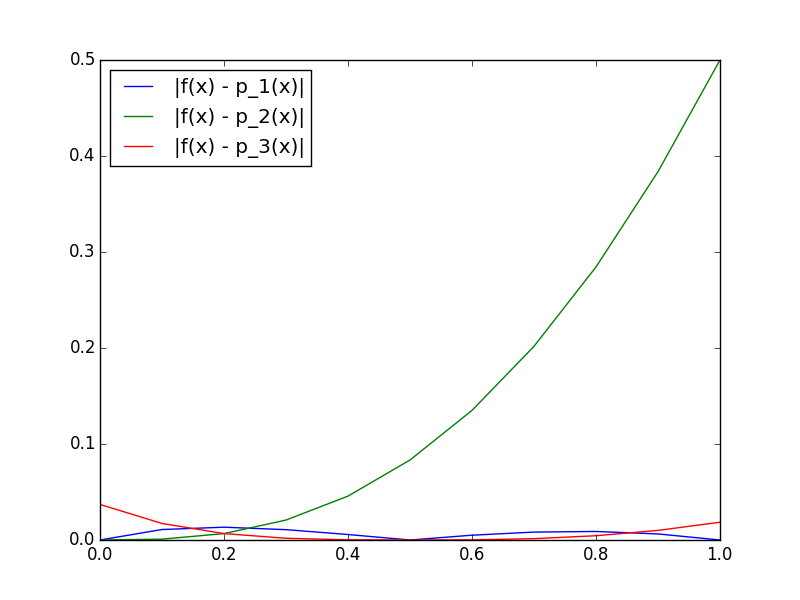
\includegraphics[scale=.6]{math_481A_lab1_figure.png}
\end{center}

\noindent Judging from the graph, $p_2(x)$ looks like the least accurate of the three parabolas, while $p_1(x)$ and $p_3(x)$ looks relatively accurate.


%\pagebreak
%\begin{thebibliography}{99}
%
%\bibitem{Abrams1997b}
%Abrams, P.~A. and Matsuda, H.
%Prey Adaptation as a Cause of Predator-Prey Cycles.
%\emph{Evolution}
%1997, 51:1742-1750.
%
%\bibitem{Chavez2001}
%Brauer, F., Castillo-Chavez, C.
%Mathematical Models in Population Biology and Epidemiology.
%Springer,
%2011. Print.
%
%\bibitem{Boyce2012}
%Boyce, W. E., and DiPrima, R. C.
%Elementary Differential Equations and Boundary Value Problems %10\textsuperscript{th} ed.
%Wiley Global Education
%2012. Print.
%
%\bibitem{Saloniemi1993}
%Saloniemi, I.
%A Coevolutionary Predator-Prey Model with Quantitative Characters.
%\emph{American Naturalist}
%1993, 141:880-896.
%
%\bibitem{Schreiber2011}
%Schreiber, S.~J., B$\ddot{\mbox{u}}$rger,  R., and Bolnick,  D.~I.
%The Community Effects of Phenotypic and Genetic Variation within a Predator %Population.
%\emph{Ecology}
%2011,  92(8):526-543. 
%
%\end{thebibliography}

\end{document}